% -------------------------------------------------------------
%		Preamble
%--------------------------------------------------------------
% !TeX spellcheck = uk_UK
%Document Settings
\documentclass[a4paper,11pt]{scrartcl}
\usepackage[T1]{fontenc}
\usepackage{setspace}
\onehalfspacing
\DeclareOldFontCommand{\bf}{\normalfont\bfseries}{\mathbf} % Includes an old command that is part of some package in here (just to make sure everything runs)

% Page numbers
\newcommand{\sectionnumbering}[1]{%
  \setcounter{section}{0}%
   \renewcommand{\thesection}{\csname #1\endcsname{section}}}

% Language settings
\usepackage[utf8]{inputenc}
\usepackage[english]{babel}

% Maths settings
\usepackage{amsmath}
\newcommand\numberthis{\addtocounter{equation}{1}\tag{\theequation}}
\usepackage{amssymb}
\usepackage{siunitx}


% Graphics packages
\usepackage{graphicx}
\graphicspath{{Graphics/}}
\usepackage{adjustbox}
\usepackage{subcaption}

% Table packages
\usepackage{pdflscape} %To create landscape environments
\usepackage{booktabs,caption}
\usepackage{threeparttable} %For nice tables
\usepackage{csvsimple} %To import excel tables 
\usepackage{import}
\usepackage{longtable}

% Bilbiography settings
\usepackage{natbib}
\bibliographystyle{apalike}

%Commenting over multiple rows
\newcommand{\comment}[1]{}



%-------------------------------------------------------------
%		Title Page
%--------------------------------------------------------------
\begin{document}

	\begin{titlepage}
		\newcommand{\HRule}{\rule{\linewidth}{0.5mm}}
		
%% Logo
	\vfill\vfill
	
\includegraphics[height=1.5cm]{UoN_Logo}\\[1cm] 


	\center			
%% Heading
	\textsc{\LARGE University of Nottingham}\\[1.5cm] 
	\textsc{\Large Applied Microeconometrics}\\[0.5cm] 	
	\textsc{\large Group Project A}\\[0.5cm] 
	
%% Title
	\HRule\\[0.4cm]
	{\huge\bfseries Insert Title}\\[0.4cm] 
	\HRule\\[0.4cm]
	
%% Date
	{\large\ Spring Term 2020} 	
	\vfill\vfill\vfill 		
	
%% Author(s) and Supervisor
\begin{flushleft}
			\large
			\textit{Supervisor}\\
			Professor Sourafel \textsc{Girma} 
			\vfill\vfill 
			\textit{Authors}\\
			Emilie \textsc{Bechtold} (20214031)\\
			Nelly  \textsc{Lehn} (20214338)\\
			Yonesse \textsc{Paris} (20115536)\\
			Georg  \textsc{Schneider} (20214032)\\
			Thea  \textsc{Zoellner} (20216019)
		\end{flushleft}
	\vfill 
	
\end{titlepage}


% -------------------------------------------------------------
%		Contents
%--------------------------------------------------------------
\pagenumbering{roman}
\sectionnumbering{Roman}
\tableofcontents

\newpage

\listoftables
\newpage

%-------------------------------------------------------------
% Main Body
%-------------------------------------------------------------
\pagenumbering{arabic}
\sectionnumbering{arabic}

\section{Introduction}


\comment{
\section{Theoretical Background/Literature Review}

\subsection{FDI}

\subsection{PSM}
Since (I guess) we will be focussing on ATE rather than ATT, we need to satisfy the following two assumptions: 

\begin{enumerate}
\item Assumption: \textbf{Unconfoundedness (CIA)} \\
"\textit{[G]iven a set of observable covariates X which are not affected by treatment, potential outcomes are independent of treatment assignment}"   \citep[p.~35]{CaliendoHujerThomsen2008}	 

\item Assumption: \textbf{Overlap} \\
"\textit{persons with the same X values have a positive probability of being both participants and nonparticipants}" \citet [p.~35]{Caliendo08}

\end{enumerate}
--> if Assumption 1 holds, all biases due to observable components can be removed by conditioning on the propensity score (Imbens, 2004).

\subsubsection*{Binary Treatment}
Difference between logit and probit lies in the link function. Logit assumes a log-distribution of residuals, probit assumes a normal distribution. Heteroskedastic probit models can account for non-constant error variances --> Check for heteroskedasticity?

\subsubsection*{Multiple Treatments}
The multinomial probit model is the preferable option compared to logit. Alternatively, just run several binary ones (more complicated but also more robust to errors).

\subsubsection*{Variable selection}
\begin{itemize}
\item outcome variable must be independent of treatment conditional on the pscore (CIA)
\item Only variables that influence simultaneously the participation decision and the outcome variable should be included (based on theory and empirical findings)
\item variables should either be fixed over time or measured before participation (include only variables unaffeted by participation)
\item choice of variables should be based on economic theory and previous empirical findings
\end{itemize}

\subsubsection*{Tests for variable selection}
Strategies for the selection of variables to be used in estimating the propensity score: ...
}

\section{Data and Descriptive Analysis}
Our analysis is based on observational firm-level data ranging from 2015 to 2017. The dataset comprises 11,323 firms, of which 4,460 received FDI in 2016. The FDI can be divided into three subcategories. Table \ref{tab:freq} shows the frequencies of each type of FDI in our sample. Among the recipients of FDI, most firms (1,965) received domestic market seeking FDI. 1,555 firms received technology intensive FDI and the remaining 640 firms received exports oriented FDI. The outcome variable TFP was measured in 2017 after the treatment. We standardize the outcome variable to a mean of zero and a standard deviation of one, to make the interpretation more intuitive. 

%--------------------TABLE 1
\begin{table}[h!]
	\centering
	\caption{Frequency of FDI Types} 
	\begin{threeparttable}
\begin{tabular}{lcc} 
	\toprule \toprule 
	FDI type&Abs. Freq.&Rel. Freq. \\[1ex]
	\midrule
	No FDI							& 6,863		& 61\% \\
	Exports oriented FDI			& 940		& 8\%	\\
	Technology intensive FDI 		& 1,555 	& 14\% 	\\
	Domestic market seeking FDI 	& 1,965 	& 17\% 	\\\\[-1.8ex]
	Total 							& 11,323 	& 100\% \\
	\bottomrule \bottomrule
\end{tabular}
\end{threeparttable}
\label{tab:freq}
\end{table}
%---------------------------

A set of categorical and continuous control variables was measured in 2015, one year prior to the firms receiving FDI. Table \ref{tab:cat} provides an overview of the categorical variables and the frequencies of each category in our sample. The categorical variables are included as factor variables in the subsequent analysis. The port variable indicates whether a firm has access to a port within 500km. The legal ownership of a firm is captured in the ownership variable. The technology intensity of the industry the respective firm is operating in, is measured in four categories from low- to high-tech. The R\&D dummy indicates whether a firm has invested in Research and Development in 2015. \\

%-------------------------TABLE 2
\begin{table}[h!]
	\centering
	\caption{Summary Statistics of Categorical Covariates} 
	\begin{threeparttable}

\begin{tabular}{lcc} \toprule \toprule 
			& Abs. Freq.	& Rel. Freq. \\
	\midrule 							\\[-1.8ex]
\textbf{Port}\textsuperscript{a} & & 						\\
No				& 7,366		& 65.05		\\
Yes				& 3,957     & 34.95		\\[1.2ex]
\textbf{Ownership}	& &					\\
Listed company	& 909 		& 8.03 		\\
Subsidiary		& 2,630 	& 23.23 	\\
Independent 	&  4,593 	& 40.56 	\\
State owned		& 3,191     & 28.18		\\[1.2ex]
\textbf{Technology Intensity}	& &		\\
Low-tech		& 4,194		& 37.04 	\\
Medium low-tech	& 1,685		& 14.88 	\\
Medium high-tech & 3,539	& 31.25 	\\
High-tech  		& 1,905		& 16.82 	\\[1.2ex]
\textbf{R\&D}\textsuperscript{b}	& &						\\
No				&  9,951	& 87.88		\\
Yes				& 1,372		& 12.12 	\\[1.2ex]
	\hline \hline
\end{tabular}

\begin{tablenotes}[flushleft]
\footnotesize
\item \textsuperscript{a} Indicates whether a firm has access to a port within 500km.
\item \textsuperscript{b} Indicates whether a firm has invested in R\&D in 2015.
\end{tablenotes}

\end{threeparttable}
	\label{tab:cat}	
\end{table}
%--------------------------------

The summary statistics of the continuous variables, i.e. wages,  total-factor productivity (TFP), firm size\footnote{Since the original variable is only available in logarithmic form and lacks an indicator for the unit of measurement we presume it is measured in number of employees.}, debts and the firms' export intensity are displayed in Table \ref{tab:cont}. The variables wages, employment and, to a lesser extent, debts show large differences between their mean and median values, hinting at the existence of outliers in the sample. Taking the logarithm of the skewed variables is an easy way of reducing the influence of extreme values. 

%-----------------------TABLE 3
\begin{table}[h!]
	\centering
	\caption{Summary Statistics of Continuous Covariates} 
	\begin{threeparttable}

\begin{tabular}{lccccc} 
\toprule \toprule
					& Mean 		& Median & Sd 		& Min 	& Max \\
\midrule \\[-1.8ex]
Wages 				& 1,967\textsuperscript{a} & 1,538 & 50,990\textsuperscript{a} & 0.00065 	& 5,519,000\textsuperscript{a} \\
TFP 				& 3.041 	& 3.032 & 2.047 	& -5.359 	& 11.36 	\\
Employment 			& 7,111 	& 81.39 & 117,155 	& 0.00197 	& 8,824\textsuperscript{a} \\
Debt 				& 1.762 	& 1.649 & 0.634 	& 0.819 	& 3.668 	\\
Export intensity 	& 0.159 	& 0.154 & 0.0798 	& 0.0103 	& 0.483 	\\\\[-1.8ex]
\bottomrule \bottomrule
\end{tabular}

\begin{tablenotes}[flushleft]
\footnotesize
\item \textit{Note:} All variables in levels.
\item \textsuperscript{a} In Thousands
\end{tablenotes}

\end{threeparttable}
	\label{tab:cont}
\end{table}
%------------------------------

However, during placebo estimation with a different outcomes it became clear that using the untransformed employment variable yields better covariate balance in all models. Noting an extreme value in this variable (see Figure \ref{fig:outliers}) we added a robustness check that excluded this observation. 
%ALTERNATIVE SUGGESTIONS: 
%However, including the log transformed employment variable deteriorates the covaraite balance in all estimated models. Despite noting at least one extreme value in this variable (see Figure \ref{fig:outliers}), we therefore include the untransformed employment variable for the estimation of our models. To rule out any bias occuring from outliers, we test the robustness of our models to the exclusion of observations with extreme values in the empolyment variable in section [ADD SECTION].

%-------------------FIGURE 1
\begin{figure}[h!]\centering
	\caption{Outliers in Employment Variable}
	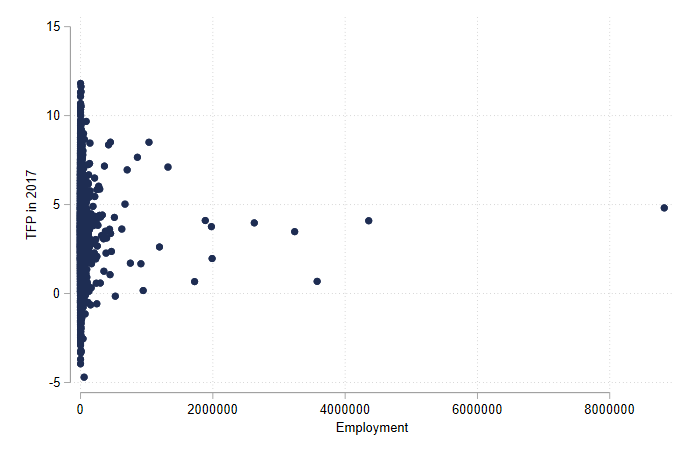
\includegraphics[width=\textwidth]{emp15_outliers}
  	\label{fig:outliers}
\end{figure} 
%---------------------------

To further motivate the use of propensity scores in estimating the effect of FDI on a firm's TFP, we show the differences in means between the firms that received FDI and the firms that did not in Table \ref{tab:meandiff1}. The t-tests show significant differences in all observable characteristics, meaning that there is in fact selection into treatment. %OR: meaning that firms are in fact chosen to receive FDI based on specific characteristics.
% If we have words left: For example, on average, FDI seems to be given to larger, more exports oriented firms. 

%-------------------------------------TABLE 4

\begin{table}[h!]
	\centering
	\caption{Difference in Pre-Treatment Covariate Means}
	\makebox[\textwidth]{
	% Balancetable grapvar(FDI2016)

\begin{threeparttable}
\begin{tabular}{lccc}
\\[-1.8ex]\toprule \toprule \\[-1.8ex]
 & (1)  & (2)  & T-test  \\
 & Control  & Treatment  & Difference (1)-(2) \\ \midrule \\[-1.8ex] 
Technology intensity & 2.565 &  1.838 	& 0.728***		\\
				& (0.014) 	& (0.015) 	& 				\\
Access to port 	& 0.273 	& 0.467 	&  -0.194***	\\ 
				& (0.005) 	& (0.007)	& 				\\
Log wages		&  7.529 	& 7.031 	& 0.498*** 		\\ 
				& (0.046)	& (0.057) 	&  				\\
TFP 			& 3.185		& 2.821		& 0.364***		\\ 
				& (0.025) 	& (0.030)  	&				\\
Log employment 	& 3.766 	& 5.405 	& -1.639***		\\
				& (0.037) 	& (0.041)  	&				\\
Log debts 		& 0.511 	& 0.493 	& 0.019***		\\ 
				& (0.004) 	& (0.005)	&			   	\\
Export intensity &  0.131 	&  0.204 	& -0.073*** 	\\ 
				& (0.001) 	& (0.001) 	&				\\
R\&D dummy 		& 0.117 	& 0.128 	& -0.012*		\\ 
				& (0.004) 	& (0.005) 	&  				\\ \\[-1.8ex]
Observations 	& 6863 		& 4460 		&				\\
\bottomrule \bottomrule 
\end{tabular} 

\begin{tablenotes}[flushleft]
\footnotesize
\item \textit{Notes}: Columns (1) and (2) show the pre-treatment covariate means of the control and treatment group respectively. Standard errors are displayed in paratheses. The values displayed for t-tests are the differences in the means across the groups. ***, **, and * indicate significance at the 1, 5, and 10 percent critical level.
\end{tablenotes}

\end{threeparttable}

}
	\label{tab:meandiff1}
\end{table}
%------------------------------------------

\newpage
\section{Empirical Specification}


We have seen in Table \ref{tab:meandiff1} that firms which received FDI differ significantly from those that did not. This indicates that treatment was not randomly assigned to firms. %Or: We have seen that FDI was not randomly assigned to firms. 
Thus, a simple comparison of treated and untreated firms will yield a biased treatment effect. Instead, we use propensity score estimation to compare the outcomes of similar firms. For this purpose we estimate the  likelihood of treatment for each firm, i.e. the propensity score. It is based on a set of observable characteristics that influence both the outcome and the likelihood of treatment. 

For the main model we use the nearest-neighbour matching estimator, which compares the outcomes of treated observations to the closest control observation in terms of propensity scores. We estimate matching models  with one and five nearest neighbours, with replacement. For the latter model we add a caliper cutoff at 0.05. We also fit inverse probability weighting models, which weigh observations by the inverse probability of being in their observed treatment group. Further, we estimate the treatment effect using the augmented inverse probability weighting model, which adds covariate adjustment to the weighting. Thus, as long as either the propensity score or the covariate adjustment model is correctly specified the results are unbiased \citep[p.~393]{imbens2015}. The point of using multiple estimators is mainly to %%CHANGE
ensure that the investigated effect is robust to the use of different estimation methods.  
% show their convergence of estimates given our large sample size. As long as results are reasonably close to each other we can take this as an indicator that the selection bias has been eliminated. (CITATION NEEDED)

%-------------
\comment{
To estimate the average causal effect of the treatment amongst all firms in the popluation we use the Average Treatment Effect (ATE) which is generally defined as: 
\begin{align*}
ATE \equiv E[Y_{i}(1)] - E[Y_{i}(0)]
\end{align*} 

where $Y_{i}(1)$ and $Y_{i}(0)$ are potential outcomes under treatment and no treatment, respectively. However we do not observe the counterfactual outcome of each firm. By just comparing outcomes of treated and untreated firms results might be biased by selection into treatment. Instead, we use for the counterfactural an estimated weighted average of the outcomes in the control group. The weights are determined by the vector of observable characteristics that determine selection into treatment. We are thus comparing like to like.  


As we face self-selection of firms into the treatment group we assume that the difference in outcome between treatment and non-treatment group are captured by a vector of observables X and the pre-entry level of the outcome variable \citep[][compare]{dehejia2002}. 
To obtain a valid control group we use "propensity score matching" method by \citet{rosenbaum1983}. This allows us to match firms which are similar in terms of their estimated propensity scores.
The probability of a firm receiving FDI $p(X_ {i}$ for is formally given by: 
\begin{align*}
p(X_{i})  \equiv  Pr(FDI_{i}|X_{i})
\end{align*} REFERENCE {DEHEJI}
We use different estimators which differ in the specification of the counterfactual by giving different weights to the matched firms. We firstly use nearest-neighbour matching with one neighbour and with replacement. Second, we estimate a nearest neighbour model with 5 neighbours with replacement and a caliper of 0.05. Further, we use  inverse probability weighting (IPW) and augmented-inverse probability weighting (AIPW) estimators. Since we have a large sample, the different estimators should all yield essentially the same results.\\}
%-------------------


 We use the same specification of covariates for the matching, weighting and regression adjustment models, unless stated otherwise. We do not include the export variable as a matching covariate, since only covariates that influence the likelihood of treatment and the outcome of interest should be included.
Although there is some debate about the direction of causality between exports and productivity, in his literature review \citet{wagner2007} argues that productivity increases exports, but not the other way around. The exclusion of the export variable significantly improves  covariate balance. We do not include the port variable for the same reason. 

Our matching model is thus a logit regression of the treatment dummy that is equal to one if the firm received FDI in 2016 on ownership, technology intensity, a Research\&Development dummy, the logarithm of wages, TFP, employment and debts in 2015. Figure \ref{fig:graph} shows evidence of sufficient propensity score overlap for a matching analysis. The covariate balance of the different models is discussed in more detail below.

%-------------------FIGURE 2
\begin{figure}[h]\centering
	\caption{Propensity Score Overlap in Main Model}
	\includegraphics[width=\textwidth]{graph}
  	\label{fig:graph}
\end{figure} 
%---------------------------


\subsection{Effect of FDI on TFP}
The main findings of this paper are displayed in Table \ref{tab:mainresults}. It reports the Average Treatment Effects of FDI on TFP. Across different estimators, we find large and highly significant coefficients, showing that receiving FDI increases TFP of companies on average. The reported coefficients differ only slightly in magnitude. 


%-------------------------------------TABLE 5
\begin{table}[h!]
 	\centering
   	\caption{ATE of FDI on TFP}
   	\label{tab:mainresults}
\begin{threeparttable}
	
 \begin{tabular}{l*{4}{c}}
	\hline
	\hline
 			& NN1 & NN5\textsuperscript{a} & IPW & AIPW \\
 			& (1) & (2) & (3)  & (4) \\ \hline
 			&  &  &  &    \\
FDI2016 	& 0.130*** & 0.114*** & 0.122***  & 0.142***   \\
 			& (0.015) & (0.011) & (0.007) &   (0.003)  \\
 	&  &  &  &    \\
PO Means 	& & & -0.068*** &  -0.057*** \\
			&  &  & (0.010)  &  (0.009) \\
			&  &  &  &    \\
 Observations & 11,323 & 11,318 & 11,323 & 11,323 \\ 
 	\hline
 	\hline 
\end{tabular}

\begin{tablenotes}[flushleft]
      \footnotesize
\item \textit{Note}: % Just a suggestion for the Tablenotes since I do think that tables should be understandable without reading the text:  
%%%NOTE: IF WE DO LEAVE THIS; TAKE OUT THE TEXTSUBSCRIPT ABOVE!
This table reports the standardized coefficients of serveral matching estimatiors. All matching was done with replacement. Columns (1) and (2) show the coefficients of the one and five nearest neighbour propensity score matching respectively. For the NN5 matching, a caliper was set to .05. Columns (3) and (4) display the coefficients of the inverse probability and augmented inverse probability matching estimators respectively.  Standard errors are displayed in paratheses. ***, **, and * indicate significance at the 1, 5, and 10 percent critical level.

%Standard errors in parentheses. *** p$<$0.01, ** p$<$0.05, * p$<$0.1.. Covariates include, unless otherwise specified: Ownership, Technology Intensity, Research\&Development, logarithm of wages, Total Factor Productivity, Employment and Debts. % Weren't we goin to leave this out?
%\item All reported coefficients are normalized for better interpretation. %all coefficients or only dependent variable? 
%\item\textsuperscript{a} We use the Propensity Score Matching method with five nearest neighbours and replacement as well as a 0.05 caliper. 
\end{tablenotes}

\end{threeparttable}
\end{table}
%------------------------------------------

Column (1) shows the results of a one-to-one propensity score matching with replacement. Receiving FDI increases productivity by 13 percent of a standard deviation for the average company. Slightly lower results are obtained from a propensity score matching with five nearest neighbors and a caliper of 0.05 in column (2) as well as for the inverse IPW in column (3). The caliper cutoff excluded five observations. The estimate of the doubly robust AIPW-estimator is slightly larger than that of the main model, but all estimates differ by no more than 3 percent of a standard deviation.

Checking the covariate balances of our models, %while the standardized differences and variance ratios are within an acceptable range for all models,%
 we prefer the one-to-one propensity score matching as it gives us the best covariate balance of all the estimators \textit{see Appendix}. %In the next subsection, we probe the sensitivity of our findings in more detail for one-to-one propensity score matching. 


\subsection{Robustness of Results}

In order to test for the sensitivity of our main findings to alternative model specifications, we perform several robustness checks for the nearest-neighbour matching estimator with one neighbour. The results are reported in Table \ref{tab:robust}. The positive and significant effect of FDI on TFP persists through all specifications, confirming our main results that foreign equity participation increases the productivity of domestic firms. 

In column (1), we add interaction terms of the dummy variables with the continuous regressors to our set of covariates. This is widely practiced to improve covariate balance \citep{Caliendo08}.
However, the covariate balance of our model does not improve with the inclusion of interaction terms, suggesting that interactions do not increase the quality of matching.\footnote{The same holds true when interacting only dummy variables, only continuous variables or all variables.} The estimated ATE of FDI on productivity slightly increases by 0.022 standard deviations compared to the effect reported in Table \ref{tab:mainresults}. 

%As we decided not to log transform the employment variable, 
Our results could further be biased by outliers of the employment variable (see Figure \ref{fig:outliers}). While most of the firms' employee numbers are concentrated around the mean of 7,111, we are concerned about two observations with extreme values: one firm with over eight million employees, and another one that apparently employed more than four million people in 2015. To check whether these outliers influence our main findings, we restrict the sample to firms with less than four million employees. The results reported in column (2) show no significant change in the treatment effect when excluding the two extreme observations. %Note% should do F-test for equality of coefficients?%
Besides, we have assumed that the presence of a port within 500 km of the firm does not influence productivity. %One could however argue that having access to a port does in fact increase productivity e.g. by facilitating access to further away markets. However, 
Column (3) reports only a small change of 0.005 standard deviations when including the port dummy in our set of covariates. 
Column (4) reports the average treatment effect on the treated (ATT) of the propensity score matching with one neighbor and replacement. While the ATE measures the average effect of FDI %on all firms, regardless of whether or not they have actually received FDI
for the hypothetical case that all firms have received FDI, the ATT only considers those firms that have actually been treated. Because it is assumed that selection into treatment is non-random, we might find stronger effects of treatment on the treated. This would be the case if those firms receiving treatment are also the ones benefiting more from it. %in terms of produtivity.
 However, our estimate in column (4) reports an ATT that is very similar to the average treatment effect. This suggests that although there was selection into treatment, the effect size would be very similar in the absence of such selection. 

 
%-----------------------TABLE 6
\begin{table}[h]
  \centering
   \caption{Robustness of Results}
   \label{tab:robust}
\begin{threeparttable}
 
\begin{tabular}{lcccc} 
	\hline 
	\hline
 		& & & & Effect \\
 		& Including & Excluding & Including & on the\\
 		& Interactions\textsuperscript{a} & Outliers\textsuperscript{b} 
 		& Port\textsuperscript{c} & Treated \\
 		& (1) & (2) & (3) & (4) \\ 
 	\hline
 		&  &  &  &  \\
ATE 	& 0.152*** & 0.127*** & 0.125*** &  \\
 		& (0.016) & (0.015) & (0.019) &  \\
 		&  &  &  &  \\
ATT 	&  &  &  & 0.127*** \\
 		&  &  &  & (0.017) \\
 		&  &  &  &  \\
Observations & 11,323 & 11,321 & 11,323 & 11,323 \\ 
	\hline
	\hline
\end{tabular}

\begin{tablenotes}[flushleft]
     \footnotesize  
 % Just a suggestion for the Tablenotes since I do think that tables should be understandable without reading the text: 
%%%NOTE: IF WE DO LEAVE THIS; TAKE OUT THE TEXTSUBSCRIPT ABOVE!     
\item \textit{Note}: All specifications are variations of our main model using the Propensity Score Matching method with one nearest neighbour and replacement. %% LEAVE THIS OUT?? %% Covariates include, unless otherwise specified: Ownership, Technology Intensity, Research\&Development, logarithm of Wages, Total Factor Productivity, Employment and Debts. 
In column (1), the main model is augmented by interactions of the dummy variables (Ownership, Technology Intensity, Research \& Development) with continuous variables (Logarithm of wages, Total Factor Productivity, Employment and Debts).  The sepcification in column (2) excludes two observations with values of Employment 2015 above four million. In column (3) we include a dummy variable indicating whether a port lies within 500km of the firm as an additional covariate. Column (4) reports the average treatment effect on the treated. Standard errors are displayed in paratheses. ***, **, and * indicate significance at the 1, 5, and 10 percent critical level. 

%\item\textsuperscript{a} Interacting dummy variables (Ownership, Technology Intensity, Research \& Development) with continuous variables (Logarithm of wages, Total Factor Productivity, Employment and Debts).  

%\item\textsuperscript{b} Two observations with extreme values of Employment 2015 above four million are excluded.
 
%\item\textsuperscript{c} Adding a dummy variable indicating whether a port lies within 500km of the firm to the set of covariates.
\end{tablenotes}

\end{threeparttable}
\end{table}
%--------------------------------------

\subsection{Treatment Effects by Technology Intensity}

FDI flows vary strongly between different sectors (see, for example, \citet{Smarzynska2004, Keller2009, Haskel2007}). In our sample, firms are divided into four industry groups, ranging from low-tech to high-tech industries. While foreign investors targeted only 13 percent of firms in high-tech industries, more than half of the observations in low-tech industries have received FDI in 2016.\footnote{See Appendix \ref{app:tech}.} This selection can have several reasons that we do not discuss in further detail.%
Instead, we focus on differences in the ATE when analyzing industries separately. 
%%CHANGE
There is in fact some empirical evidence for heterogeneity of the effect of FDI on firm productivity depending on a firm's technology intensity. 
%%
For instance, \citet{Keller2009} find a strong effect of FDI on the productivity of domestically owned firms in the high-tech sector but only a very small, if any, effect on low-tech industries. Table \ref{tab:TECH}, reports the estimates of the ATE of FDI on productivity separately for each industry. Standard errors have increased slightly, but the results are still highly significant. 

%-----------------------TABLE 7
\begin{table}[h!]
  \centering
   \caption{ATE by Technology Intensity of Industry}
   \label{tab:TECH}
\begin{threeparttable}
 
\begin{tabular}{lcccc}
 \hline
 \hline
 & & Medium & Medium &  \\ 
 & Low-Tech & Low-Tech & High-Tech & High-Tech \\ 
 & Industry & Industry & Industry & Industry \\ 
 & (1) & (2) & (3) & (4) \\
 \hline
 &  &  &  &  \\
FDI2016 & 0.160*** & 0.086*** & 0.172*** & 0.180*** \\
	      & (0.020) & (0.028) & (0.019) & (0.054) \\
	      &  &  &  &  \\
 Observations & 4,194 & 1,685 & 3,539 & 1,905 \\ 
	\hline
	\hline
\end{tabular}	

\begin{tablenotes}[flushleft]
     \footnotesize     
% Another notes suggestion   
\item \textit{Note}: The table reports the standardized ATE coefficients for subsamples of firms with different levels of technology intensitiy. Standard errors are displayed in paratheses. ***, **, and * indicate significance at the 1, 5, and 10 percent critical level. 

\end{tablenotes}


\end{threeparttable}
\end{table}
%--------------------------------------

The impact of FDI does indeed vary across industries. Our estimates support the finding of \citet{Keller2009} that firms in high-tech industries benefit the most, as FDI increases productivity of these firms by 18 percent of a standard deviation, five percentage points more than our results for the full sample would suggest. Somewhat surprising is that the estimates for the low-tech industry are also higher than in our main specification. The medium low-tech industry instead does not benefit as much as the other industries do. It experiences an increase in TFP of only 8.6 percent of a standard deviation when receiving FDI. 
%An F-test rejects the null hypothesis of equality of the ATE between industries. (Probably, if I figured out how to do it...)
\\
The weighted average of these estimates yields an ATE of FDI on TFP of 0.158 standard deviations.\footnote{Weights are allocated according to relative sample size.} This effect slightly differs from our main result due to the fact that matching is now performed within industry only. Although matched neighbours might be more 'distant' regarding other covariate values, we can ensure that each treated firm is allocated to a control observation with the same technology intensity. The covariate balances remain very good. 


\section{Analysis by Type of FDI}

To further test the robustness of our results, we continue our analysis by looking at potential heterogeneity of the treatment effect across types of FDI. %%Really don't think we need this again.%% Recall the three types of FDI from Table \ref{tab:bytype} as Exports oriented, Technology intensive and Domestic market seeking, with the the latter being most common and the first being least common.
We test the possibility that one specific type of investment single handedly drives our previous results. It is possible that, for example, only exports-oriented FDI increases factor productivity while the other two types have little or no impact. 

We estimate an augmented IPW model with multi-valued treatment effects. The matching covariates are the same as in the previous model and the regression adjustment specification is the same as that for propensity score estimation. The covariate balance is good, but the variance ratio of employment (unlogged) is a borderline case. \footnote{Unfortunately an AIPW model with any interactions did not converge, so it was impossible to try and improve the balance this way.}%footnote sounds a bit like we failed in our analysis. 

We further estimate an IPW model to check if it yields similar estimates without regression adjustment. The covariate balance in this model is practically the same. Finally, we specify a set of AIPW models where we restrict the sample to one type of treatment each. This allows for the IIA assumption to be relaxed which is required for the mulitnominal logit models. The separate models have worse covariate balance than the first two but are borderline acceptable. The overlap assumption is satisfied for all treatment levels as can be seen in Figure \ref{fig:over_typ}. 


In Table \ref{tab:bytype} the results from the type-wise analysis are shown. In the AIPW Multinomial specification the ATE of different types of FDI are within half a percent of of each other. This suggests, that all types of FDI increase factor productivity by essentially the same margin. The estimated effect size is close to the one estimated for FDI in table 2. In the IPW specification the differences slightly larger but still within 5\% of a standard deviation of each other.  The separate logit models also yield essentially the same effect sizes as the multinomial specification. Since the AIPW estimator is doubly robust (assuming correctly specified regression adjustment models) models (1) and (3) provide us with strong evidence of homogenous effects.


%-------------------FIGURE 2
\begin{figure}[h]
	
	\caption{Propensity Score by Treatment Level}
\hspace*{-2cm}  	
	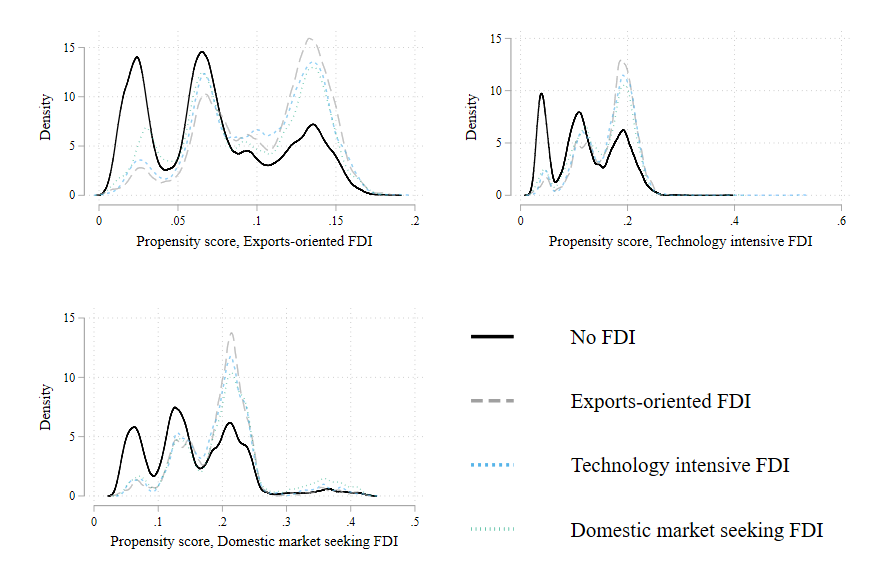
\includegraphics[height=12cm]{overlap_type.png}\\ 
	\label{fig:over_typ}
 
\end{figure}
%---------------------------



%-----------------------------TABLE 8
\begin{table}[htbp]
	\centering
	\caption{ATE by Type of FDI}
	\label{tab:bytype}
\begin{threeparttable}

\begin{tabular}{lccccc} 
		\hline
		\hline
 	& (1) & (2) & (3) & (4) & (5) \\
	& AIPW & IPW  & AIPW  & AIPW & AIPW \\ 
	& Mlogit & Mlogit &Logit &Logit &Logit\\
		\hline
 			&  &  &  &  &   \\
Exports-oriented FDI 	& 0.144*** &   0.157*** & 0.140*** &  &  \\
 						& (0.006) &   (0.032) & (0.007) &  &\\ \\[-1.8ex]
Technology intensive FDI & 0.139***   & 0.112*** &  & 0.139*** &   \\
 						 & (0.005)  & (0.018) &  &  (0.005)&  \\ \\[-1.8ex]
Domestic market seeking FDI & 0.143*** &   0.134*** &  &  &0.143*** \\
 							& (0.004)   & (0.011) &  &  & (0.004)  \\ \\[-1.8ex]
PO Means 		&   -0.057*** &   -0.068*** &-0.012  &-0.025**  & -0.017    \\
 				&   (0.009) &   (0.010) &  (0.011)&(0.011)  & (0.011) \\ \\[-0.2em]
Observations 	& 11,323  & 11,323 &  7,803  & 8,418 & 8,828  \\ 
		\hline
		\hline
\end{tabular}

%Another tablenote suggestion
\begin{tablenotes} [flushleft]
\footnotesize
\item \textit{Note:} Columns (1) and (2) report the coefficients of the multinominal augmented inverse probability and multinominal inverse probability matching estimators respectively. Columns (3)-(5) display the results of the augmented inverse probability matching estimator for subsamples of firms having received different types of FDI. Standard errors are displayed in paratheses. ***, **, and * indicate significance at the 1, 5, and 10 percent critical level. 
\end{tablenotes}

\end{threeparttable}
\end{table}
%------------------------------------------------


\section{Discussion/Conclusion}

%--------------how to cite
\comment{
For citation: \\
you have to add your reference firstly in bibCG. After having done so you can always include the reference in the actual file as follows: \\
 \citet{aitken99}\\
\citep[p.~35]{CaliendoHujerThomsen2008}	}
%--------------

Thoughts on what we could write for discussion/limits of our study: 
\begin{enumerate}
\item Do not know much about the context of the treatment (so cannot really rule out anticipation-effects?)
\item Would have been interesting to extend the study to several years after the treatment. Do effects persist? Do they vanish? 
\item Might depend on firm size (see \citet{aitken99}): find positive within-plant effects and spillover effects on TFP for small firms only (less than 50 employees)
\item Do not measure spillovers on plants that have not received FDI
\item Do not have sector-specific data $\rightarrow$ TECH variable has only 4 categories; e.g. in order to measure spillover effects from other firms in sector this would be necessary (i.e. if a foreign firm is more innovative)
\end{enumerate}

%maybe in conclusion/ limits of paper
One shortcoming of our analysis is the missing capability to explain the mechanisms behind the observed treatment effects. We do not distinguish between within-firm effects and spillover effects from firms receiving FDI to other firms. That is, the literature on spillover effects typically suggests spillovers within sectors rather than across sectors (SOURCE) and higher spillover effects on nearby firms or firms that are trading factor inputs with foreign-owned companies (SOURCE). Due to the limited information on a firm's sector and location, we are unable to measure spillover effects. 

\newpage

%-------------------------------------------------------------
% References
%-------------------------------------------------------------
\addcontentsline{toc}{section}{References}	%Adds references to table of contents
\bibliography{bibCG} 
\newpage


%-------------------------------------------------------------
% Appendix
%-------------------------------------------------------------
\pagenumbering{roman}
\sectionnumbering{Roman}
\setcounter{page}{3} %May have to adjust this if we leave out list of tables or add something else

\appendix
\section{Appendix}

%---------------------------FDI BY TECH (ROBUSTNESS)
\subsection{Treatment by Technology Intensity}
\label{app:tech}
\begin{table}[htbp]
	\centering
\begin{threeparttable}

\begin{tabular}{lcccccc} 
\hline
\hline
 & \multicolumn{6}{c}{FDI in 2016} \\
Technology intensity & \multicolumn{3}{c}{No} & \multicolumn{3}{c}{Yes} \\
of industry &No.&Col \% &Cum \% &No.&Col \% &Cum \% \\
\hline
	&  &  &  &  &  &   \\
Low-tech &1869&44.6&27.2&2325&55.4&52.1 \\
Medium low-tech &904&53.6&40.4&781&46.4&69.6 \\
Medium high-tech &2432&68.7&75.8&1107&31.3&94.5 \\
High-tech &1658&87.0&100.0&247&13.0&100.0 \\
\textbf{Total}&\textbf{6863}&\textbf{60.6}&&\textbf{4460}&\textbf{39.4}& \\
\hline
\hline
\end{tabular}

\end{threeparttable}
\end{table}
%-----------------------------------

\end{document}